\input{../latex-math/basic-math}
\input{../latex-math/basic-ml}
\input{../latex-math/ml-nn}

\begin{document}

\lecturechapter{6}{Basic Training}
\lecture{Basic Training}
%%%%%%%%%%%%%%%%%%%%%%%%%%%%%%%%%%%%%%%%%%%%%%%%%%%%%%%%%%%%%%%%%%

\begin{vbframe}{Training Neural Networks}
\lz
Training of neural nets is composed of two iterative steps:
\lz
\begin{enumerate}
\item \textbf{Forward pass:} The information of the inputs flows through the model to produce a prediction. Based on this prediction, the empirical loss is computed.
\lz
\item \textbf{Backward pass:} The information of the prediction error flows backward through the network to update the weights in a way that the error reduces.
\end{enumerate}
\lz

\textbf{Recall:} The error is calculated via a loss function $L(y, f(x, \thetab))$, where $y$ and $f(x, \thetab)$ are the true target and the network outcome respectively.
\framebreak
%%%%%%%%%%%%%%%%%%%%%%%%%%%%%%%%%%%%%%%%%%%%%%%%%%%%%%%%%%%%%%%%%%

\lz
\lz
\begin{itemize}
\item For regression, the L2 loss is typically used:
$$\Lxy = \frac{1}{2}(y - \fx)^2$$
\item For classification, the binary/categorical cross entropy:
$$\Lxy = y \log \fx + (1 - y) \log(1 - \fx)$$
\end{itemize}
\lz
\lz
\textbf{Note:} Evaluated the loss on the data, the \textbf{risk function} is computed:
$$\riske = \sumin \Lxyi$$
\framebreak
%%%%%%%%%%%%%%%%%%%%%%%%%%%%%%%%%%%%%%%%%%%%%%%%%%%%%%%%%%%%%%%%%%

\lz
To minimize the risk, the \textbf{gradient descent} (GD) method can be used.
\lz
\begin{itemize}
\item First, we calculate the gradient $\nabla \risk$ at a point $\theta^{[t]}$.
\lz
\item \enquote{Standing} at $\thetab^{[t]}$, we then improve the minimization by performing the following update:
$$\thetab^{[t + 1 ]}  = \thetab^{[t]} - \alpha \nabla \risk\left(\thetab^{[t]}\right).$$
\item $\alpha$ determines the length of the step and is called the \textbf{learning rate}.
\end{itemize}
\lz
\lz
\textbf{Note:} Since $\nabla \risk$ always points in the direction of the steepest ascent, $-\nabla \risk$ always points in the direction of the steepest descent!
\end{vbframe}
%%%%%%%%%%%%%%%%%%%%%%%%%%%%%%%%%%%%%%%%%%%%%%%%%%%%%%%%%%%%%%%%%%

\begin{vbframe}{Example: Gradient descent}
\begin{center}
\begin{figure}
\centering
\scalebox{1}{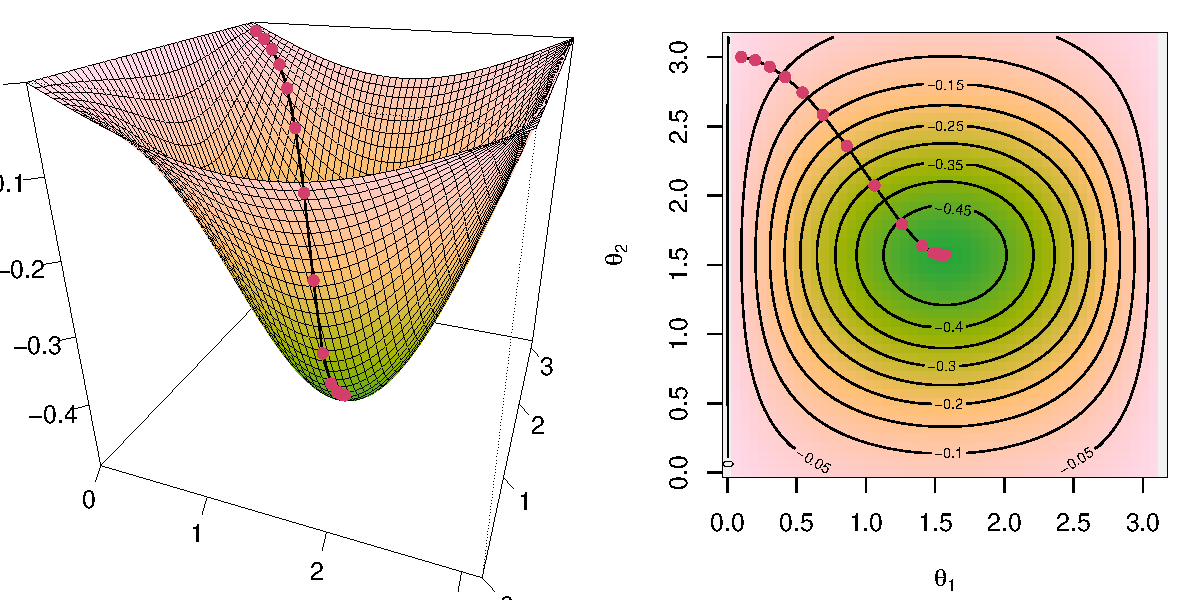
\includegraphics{../plots/hill.pdf}}
\end{figure}
\vspace{1 cm}
"Walking down the hill, towards the valley."
\end{center}
\end{vbframe}
%%%%%%%%%%%%%%%%%%%%%%%%%%%%%%%%%%%%%%%%%%%%%%%%%%%%%%%%%%%%%%%%%%

\begin{vbframe}{Weight updates with Backpropagation}
\begin{itemize}
\lz
\item To update each weight $w \in \thetab$ in the network, we need their gradients with regards to the risk.
\lz
\lz
\item Since weights are stacked in layers inside the network, we need to repeatedly apply the \enquote{chain rule of calculus}. This process is called \textbf{backpropagation}.
\lz
\lz
\item After obtaining the gradients, the weights can be updated by GD:
$$\thetab^{[t + 1]} = \thetab^{[t]} - \alpha \cdot \frac{1}{n} \cdot \sumin \nabla_\theta L\left(\yi, f(\xi ~|~ \thetab^{[t]})\right)$$
\end{itemize}
\end{vbframe}
%%%%%%%%%%%%%%%%%%%%%%%%%%%%%%%%%%%%%%%%%%%%%%%%%%%%%%%%%%%%%%%%%%

\begin{vbframe}{Stochastic Gradient Descent}
\begin{itemize}
\lz
\item Optimization algorithms that use the entire training set to compute updates in one huge step are called \textbf{batch} or \textbf{deterministic}. This is computationally very costly or often impossible.
\lz
\item Instead of running the sum over the whole dataset (\textbf{batch mode}), one can run over small subsets (\textbf{minibatches}) of size $m$.
\lz
\item With minibatches of size $m$, a full pass over the training set (called an \textbf{epoch}) consists of $\frac{n}{m}$ gradient updates.
\lz
\item This stochastic version of the batch gradient is known as \textbf{Stochastic Gradient Descent} (SGD).
\end{itemize}
\framebreak
%%%%%%%%%%%%%%%%%%%%%%%%%%%%%%%%%%%%%%%%%%%%%%%%%%%%%%%%%%%%%%%%%%

An illustration of the SGD algorithm: on the left is GD and on the right is SGD. The black line depicts the averaged value of $\thetab$.

\begin{figure}
\scalebox{1}{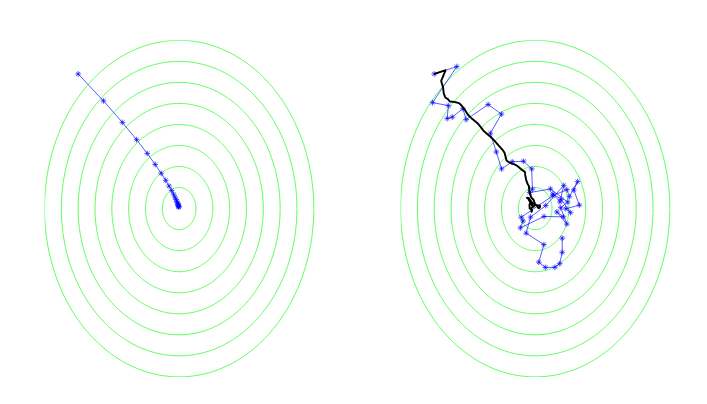
\includegraphics{../plots/SGD.png}}
\tiny{\\ source : Shalev-Shwartz and  Ben-David.
Understanding machine learning: From theory to algorithms. Cambridge University Press, 2014.}
\end{figure}
\framebreak
%%%%%%%%%%%%%%%%%%%%%%%%%%%%%%%%%%%%%%%%%%%%%%%%%%%%%%%%%%%%%%%%%%

  \begin{algorithm}[H]
  \footnotesize
    \caption{Basic SGD pseudo code}
    \begin{algorithmic}[1]
    \State Initialize parameter vector $\thetab^{[0]}$
    \State $t \leftarrow 0$
    \While{stopping criterion not met}
    \State Randomly shuffle data and partition into minibatches $J_1, ..., J_K$ of size $m$
      \For{$k\in\{1,...,K\}$}
      \State $t \leftarrow t + 1$
      \State Compute gradient estimate with $J_k$:
      \[\hat{g}^{[t]} \leftarrow \frac{1}{m} \sum_{i \in J_k} \nabla_\theta L(\yi, f(\xi ~|~ \thetab^{[t-1]}))
      \]
      \State Apply update: $\thetab^{[t]} \leftarrow \thetab^{[t-1]} - \alpha \hat{g}^{[t]}$
      \EndFor
      \EndWhile
    \end{algorithmic}
  \end{algorithm}
\end{vbframe}
%%%%%%%%%%%%%%%%%%%%%%%%%%%%%%%%%%%%%%%%%%%%%%%%%%%%%%%%%%%%%%%%%%

\begin{vbframe}{SGD with Momentum}
\begin{itemize}
\item While SGD remains a popular optimization strategy, learning with it can sometimes be slow.
\item Momentum is designed to accelerate learning, by accumulating an exponentially decaying moving average of past gradients.
\end{itemize}
\begin{figure}
\centering
\scalebox{.8}{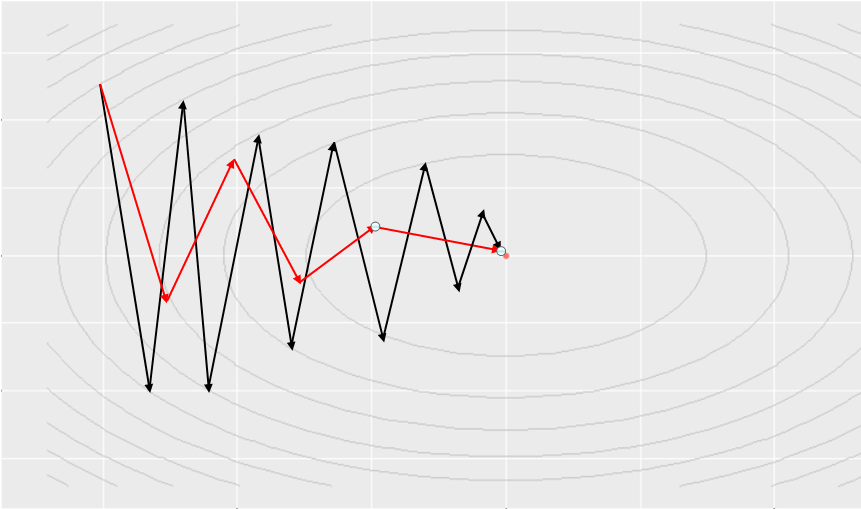
\includegraphics{../plots/momentum.png}}
\\GD (black) versus momentum (red) when dealing with ravines
\end{figure}
\end{vbframe}
%%%%%%%%%%%%%%%%%%%%%%%%%%%%%%%%%%%%%%%%%%%%%%%%%%%%%%%%%%%%%%%%%%

\endlecture
\end{document}